\documentclass[pdftex,12pt,a4paper]{article}

\usepackage{graphicx}  
\usepackage[margin=2.5cm]{geometry}
\usepackage{breakcites}
\usepackage{indentfirst}
\usepackage{pgfgantt}
\usepackage{pdflscape}
\usepackage{float}
\usepackage{epsfig}
\usepackage{epstopdf}
\usepackage[cmex10]{amsmath}
\usepackage{stfloats}
\usepackage{multirow}
\usepackage{listings}
\lstdefinestyle{customc}{
  belowcaptionskip=1\baselineskip,
  breaklines=true,
  frame=L,
  xleftmargin=\parindent,
  language=Verilog,
  showstringspaces=false,
  basicstyle=\footnotesize\ttfamily,
  keywordstyle=\bfseries\color{green!40!black},
  commentstyle=\itshape\color{purple!40!black},
  stringstyle=\color{orange},
}

\lstdefinestyle{customasm}{
  belowcaptionskip=1\baselineskip,
  frame=L,
  xleftmargin=\parindent,
  language=[x86masm]Assembler,
  basicstyle=\footnotesize\ttfamily,
  commentstyle=\itshape\color{purple!40!black},
}
\lstset{escapechar=@,style=customc}


\renewcommand{\refname}{REFERENCES}
\linespread{1.3}
\usepackage{mathtools}

%\newcommand{\HRule}{\rule{\linewidth}{0.5mm}}
\thispagestyle{empty}
\begin{document}
\begin{titlepage}
\begin{center}
\textbf{}\\
\textbf{\Large{ISTANBUL TECHNICAL UNIVERSITY}}\\
\vspace{0.5cm}
\textbf{\Large{COMPUTER ENGINEERING DEPARTMENT}}\\
\vspace{2cm}
\textbf{\Large{BLG 242E\\ DIGITAL CIRCUITS LABORATORY\\ EXPERIMENT REPORT}}\\
\vspace{2.8cm}
\begin{table}[ht]
\centering
\Large{
\begin{tabular}{lcl}
\textbf{EXPERIMENT NO}  & : & 3 \\
\textbf{EXPERIMENT DATE}  & : & 01.04.2021 \\
\textbf{LAB SESSION}  & : & FRIDAY - 14.00 \\
\textbf{GROUP NO}  & : & G4 \\
\end{tabular}}
\end{table}
\vspace{1cm}
\textbf{\Large{GROUP MEMBERS:}}\\
\begin{table}[ht]
\centering
\Large{
\begin{tabular}{rcl}
150180086  & : & EFE YİĞİT TAŞ \\
150170050  & : & MERT  YEREKAPAN \\
150180008  & : & LAL VERDA ÇAKIR \\
\end{tabular}}
\end{table}
\vspace{2.8cm}
\textbf{\Large{SPRING 2021}}

\end{center}

\end{titlepage}

\thispagestyle{empty}
\addtocontents{toc}{\contentsline {section}{\numberline {}FRONT COVER}{}}
\addtocontents{toc}{\contentsline {section}{\numberline {}CONTENTS}{}}
\setcounter{tocdepth}{4}
\tableofcontents
\clearpage

\setcounter{page}{1} 

\section{INTRODUCTION [10 points]}
In this experiment we implement 16-Bit Full Adder-Subtractor  using 4-bit Full adder and 1-bit Full adder.Since we implemented 16-Bit Full Adder-Subtractor in this way, we learned about the working system of 16-bit full adder. We also observed in which cases overflow occurs.

\section{MATERIALS AND METHODS [40 points]}

\subsection{PART 1}
In this part we implemented AND, OR, NOT and XOR gates to use in the future.

Firstly we implemented NOT gate. The shematics of the NOT gate has shown below.

\begin{figure}[H]
	\centering
	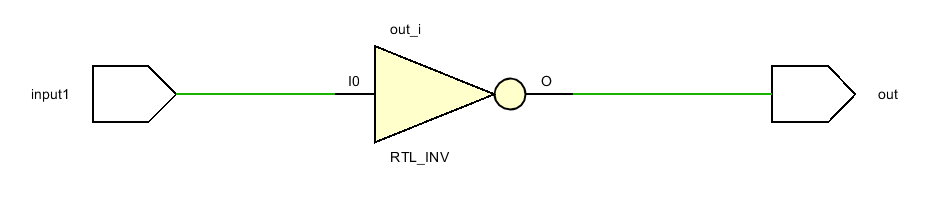
\includegraphics[width=0.75\textwidth]{not_gate_vivado.png}	
	\caption{NOT Gate}
	
\end{figure}

Then we implemented OR gate. The shematics of the OR fate has shown below.

\begin{figure}[H]
    \centering
    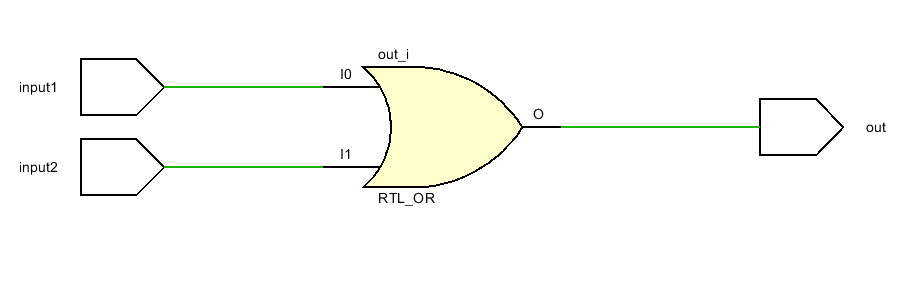
\includegraphics[width=0.75\textwidth]{or_gate_vivado.png}
    \caption{OR Gate}
\end{figure}

Then we implemented AND gates. For the following parts we need 2 and 3 inputed AND gates so we implemented both of them. You can see the schematics below.

\begin{figure}[H]
    \centering
    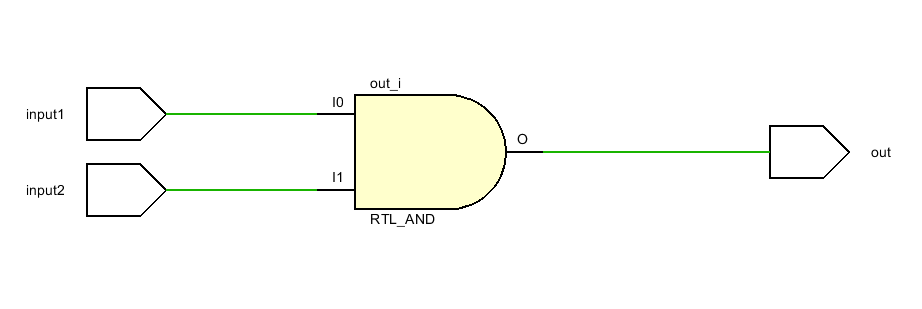
\includegraphics[width=0.75\textwidth]{andgate_viado.png}
    \caption{2 Input AND Gate}
\end{figure}
\begin{figure}[H]
    \centering
    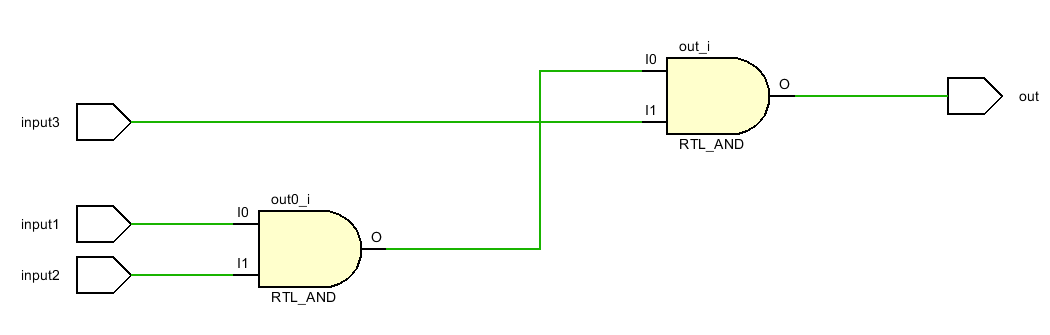
\includegraphics[width=0.75\textwidth]{andgate3input_vivado.png}
    \caption{3 Input AND Gate}
\end{figure}

And finally we need XOR gate. Schematics of XOR gate has shown below.

\begin{figure}[H]
    \centering
    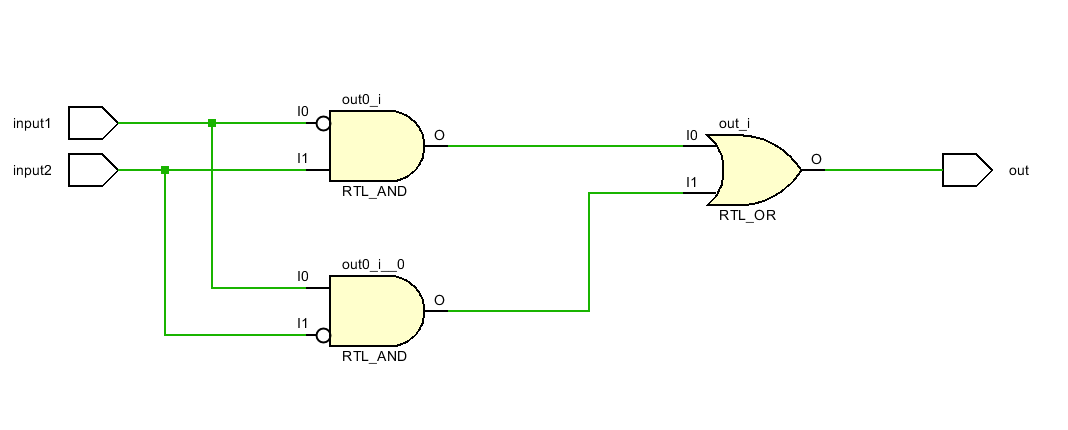
\includegraphics[width=0.75\textwidth]{xor_gate_vivado.png}
    \caption{XOR Gate}
\end{figure}

\subsection{PART 2}

In this part we implemented 1-bit half adder using AND, OR, NOT and XOR modules which we designed in first part. Schematics of the half adder is below. 
\begin{figure}[H]
    \centering
    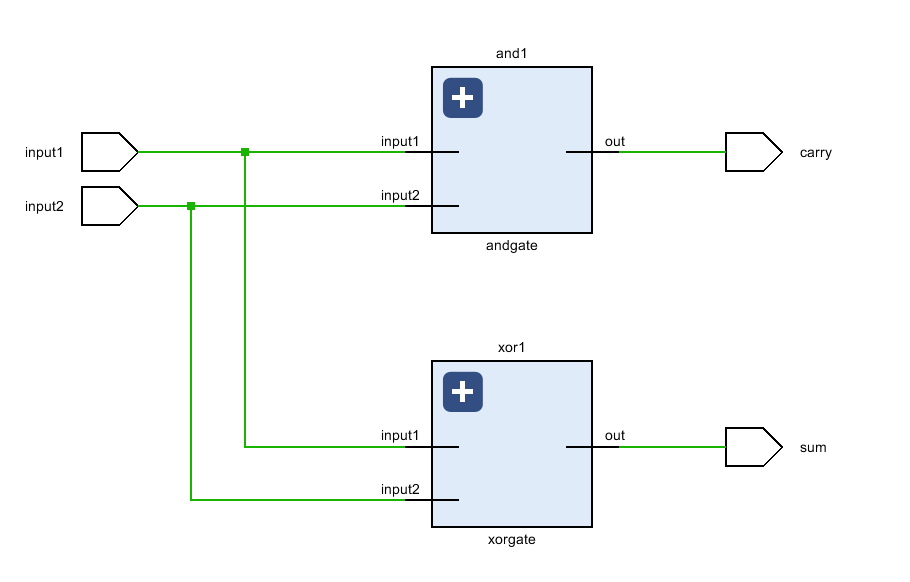
\includegraphics[width=0.5\textwidth]{halfadder_vivado.png}
    \caption{1-Bit Half Adder}
\end{figure}

\subsection{PART 3}

In this part we implemented 1-bit full adder using 2 half adders and 1 OR gate which we designed in first and second part. We can see that the only difference from Half-Adder is the $C_i_n$ input.

\begin{figure}[H]
    \centering
    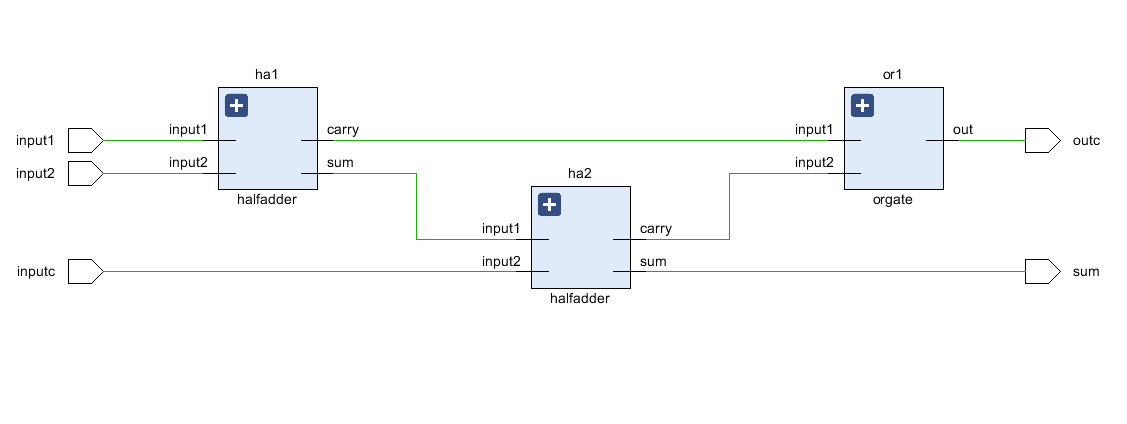
\includegraphics[width=0.75\textwidth]{fulladder_vivado.png}
    \caption{1-Bit Full Adder}
\end{figure}

\subsection{PART 4}

In this part we implemented 4-bit full adder using 4 1-bit full adders which we designed in previous part. The difference of this part from the previous part is that the input and output are 4 bits.


\begin{figure}[H]
    \centering
    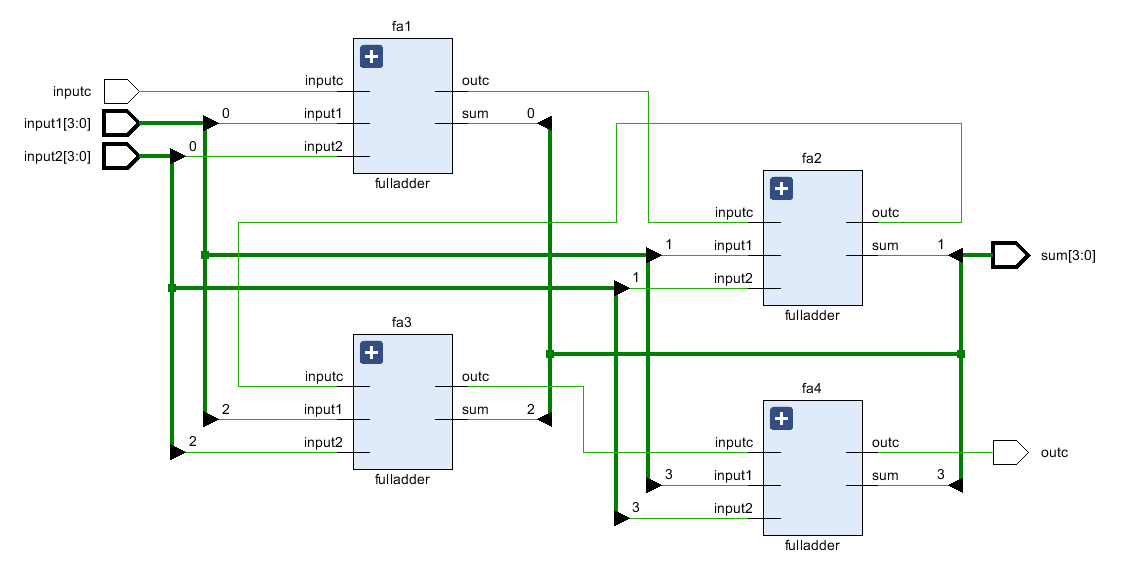
\includegraphics[width=0.5\textwidth]{fulladder4bit_vivado.png}
    \caption{4-Bit Full Adder}
   
\end{figure}

\subsection{PART 5}

In this part we implemented 16 bit full adder using 4 bit full adders. The difference of this part from the previous part is that the input and output are 16 bits.

\begin{figure}[H]
    \centering
    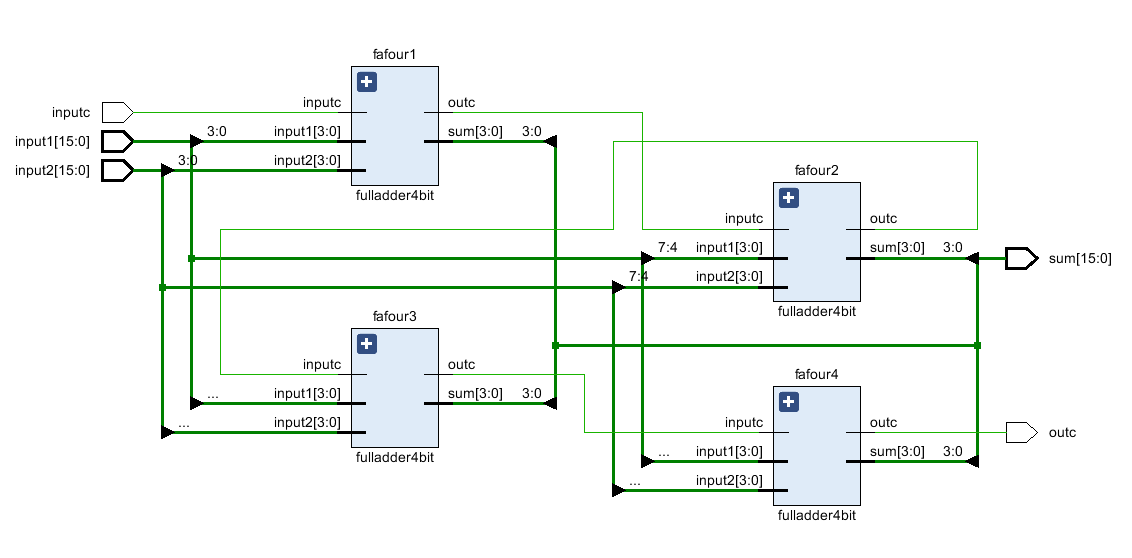
\includegraphics[width=0.5\textwidth]{fulladder16bit_vivado.png}
    \caption{16-Bit Full Adder}
\end{figure}

\subsection{PART 6}

In this part we implemented 16-bit adder substractor that works on both signed and unsigned integers. We also implemented the circuit that shows in which cases overflow occurs.

\begin{figure}[H]
    \centering
    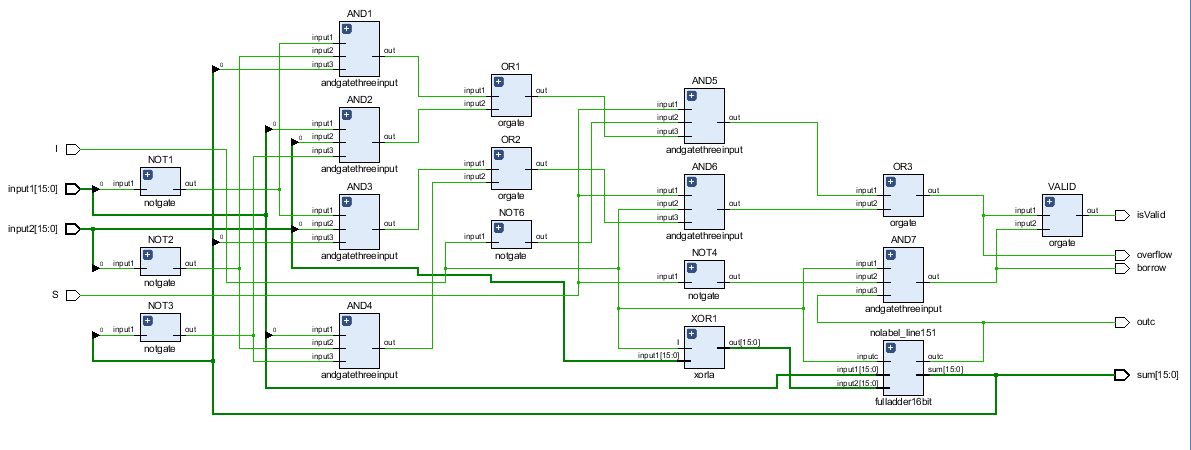
\includegraphics[width=0.5\textwidth]{adder_substractor_vivadı.png}
    \caption{16-Bit Adder/Substractor}
\end{figure}

\subsection{PART 7}

In this part we implemented calculator module which calculates 3A-2B for any given 16-bit A and B.

\begin{figure}[H]
    \centering
    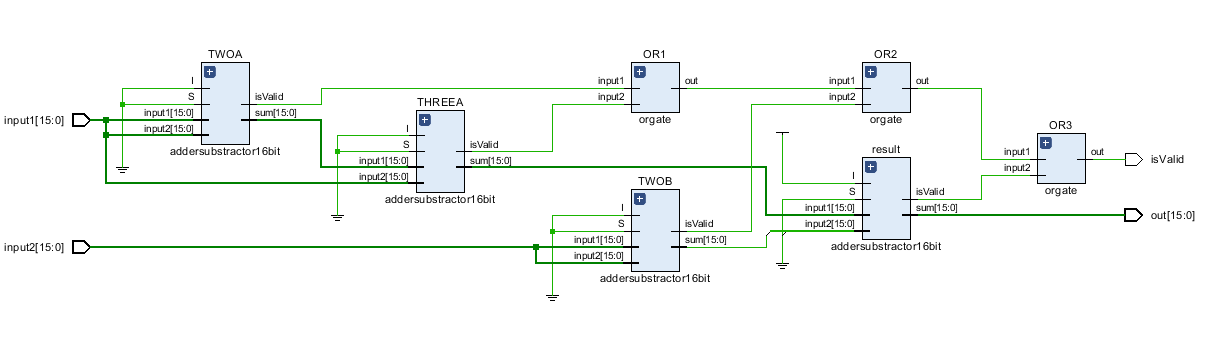
\includegraphics[width=0.5\textwidth]{part7_verilog.png}
    \caption{16-Bit 3A-2B calculator}
\end{figure}

\section{RESULTS [15 points]}
\subsection{PART 1}
In this part we tested 2 input AND,3 input AND, OR, NOT and XOR gates using bit-wise operations; \&(and), $|$ (or), \texttildelow (not). We checked the output of each simulations to see if our function correctly. Figure 10 and Figure 11 shows the 2 input and 3 input AND gates simulation results, Figure 12 shows the OR gate simulation result, Figure 13 shows the NOT gate simulation result and Figure 14 shows the XOR gate simulation result.

\begin{figure}[H]\label{fig6}
	\centering
	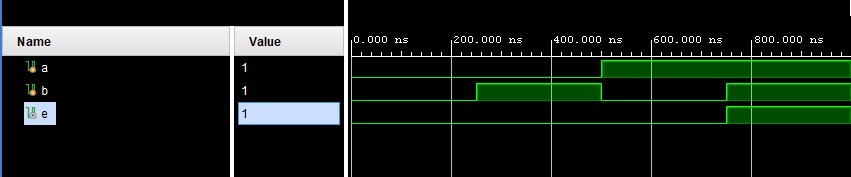
\includegraphics[width=0.5\textwidth]{and_gate_result.jpeg}	
	\caption{Simulation Result of the 2 input AND Gate}
	
\end{figure}
\begin{figure}[H]\label{fig6}
	\centering
	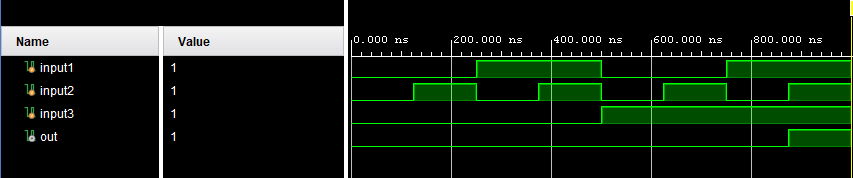
\includegraphics[width=0.5\textwidth]{andgate3input_sim.png}	
	\caption{Simulation Result of the 3 input AND Gate}
	
\end{figure}
\begin{figure}[H]
	\centering
	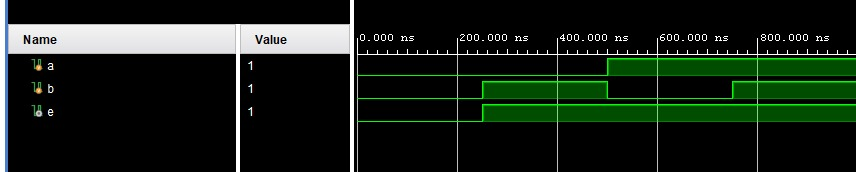
\includegraphics[width=0.5\textwidth]{or_gate_result.jpeg}	
	\caption{Simulation Result of the OR Gate}
	\label{fig7}
\end{figure}
\begin{figure}[H]
	\centering
	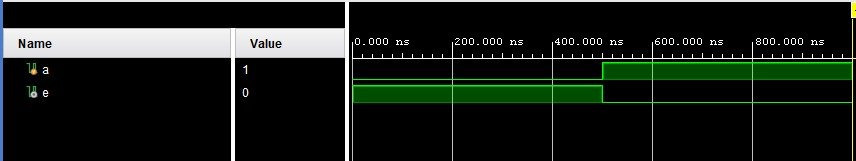
\includegraphics[width=0.5\textwidth]{not_gate_result.jpeg}	
	\caption{Simulation Result of the NOT Gate}
    \label{fig8}
\end{figure}
\begin{figure}[H]
	\centering
	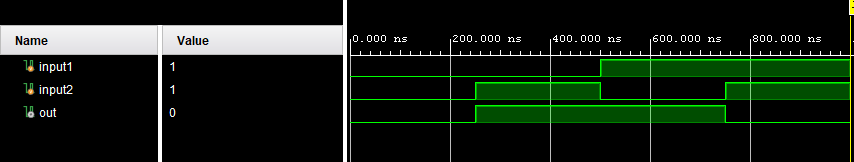
\includegraphics[width=0.5\textwidth]{xorgate_sim.png}	
	\caption{Simulation Result of the XOR Gate}
    \label{fig8}
\end{figure}
\subsection{PART 2}
In this part we tested the half adder we designed using AND, OR, NOT and XOR modules which we designed in first part. Simulation results in Figure 16.
\begin{figure}[H]
    \centering
    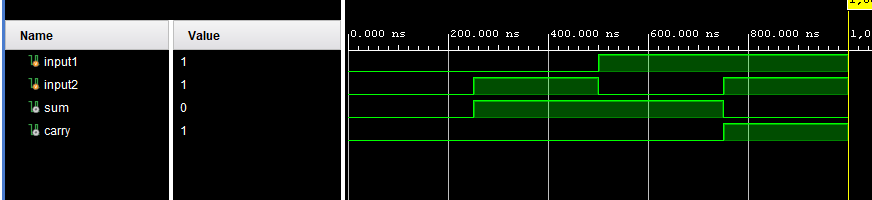
\includegraphics[width=0.5\textwidth]{halfadder_sim.png}
    \caption{1-Bit Half Adder Simulation}
\end{figure}
\subsection{PART 3}
In this part we tested full adder we designed by using half adder and OR modules which we designed in first and second part. As you can see from the simulation results in Figure 17, the only difference from Half-Adder is the $C_i_n$ input.

\begin{figure}[H]
    \centering
    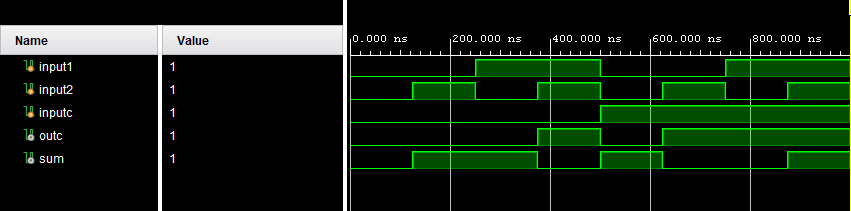
\includegraphics[width=0.5\textwidth]{fulladder_sim.png}
    \caption{1-Bit Full Adder Simulation}
\end{figure}

\subsection{PART 4}

In this part we tested 4-bit full adder we designed using 1-Bit Full Adder modules which we designed in the previous part. As you can see in Figure 18, this simulation result looks a little different from the previous results because our output and input are 4 bits.


\begin{figure}[H]
    \centering
    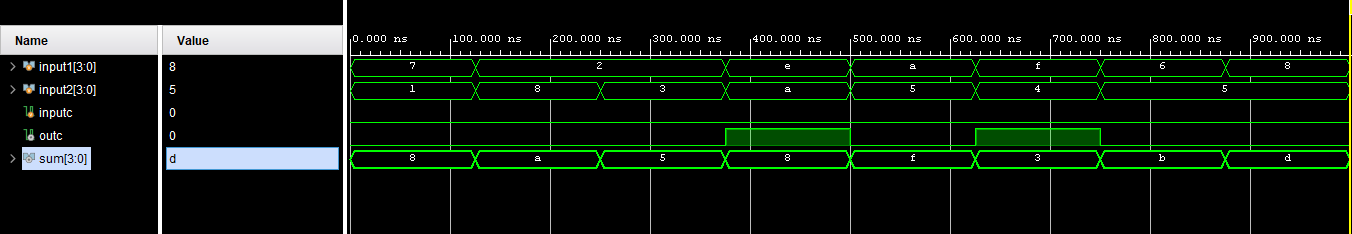
\includegraphics[width=0.5\textwidth]{fulladder4bit_sim.png}
    \caption{4-Bit Full Adder Simulation}
\end{figure}

\subsection{PART 5}

In this part we tested 16-bit full adder we designed using 4-Bit Full Adder modules which we designed in the previous part. The only difference of this stage from PART 4 is that the inputs and outputs are 16 bits.


\begin{figure}[H]
    \centering
    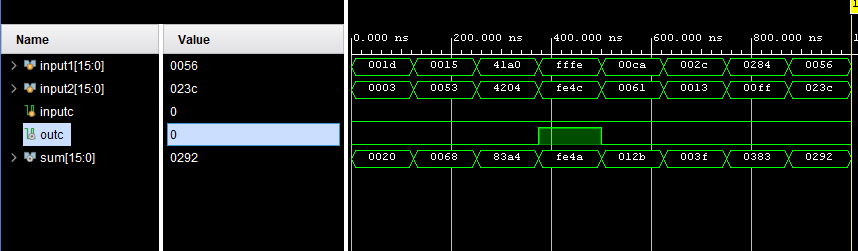
\includegraphics[width=0.5\textwidth]{fulladder16bit_sim.png}
    \caption{16-Bit Full Adder Simulation}
\end{figure}
\newpage

\subsection{PART 6}

In this part we tested 16-bit adder/substractor we designed using 16-Bit Full Adder, NOT, XOR, AND, and OR modules which we designed in the previous parts. As a result of the simulation you see in Figure 20, we see not only what the output is but also the situations where overflow occurs.


\begin{figure}[H]
    \centering
    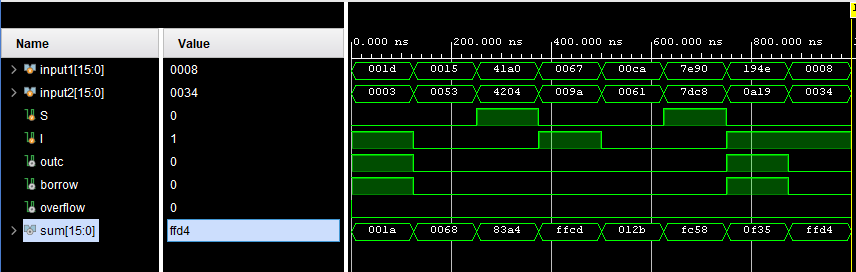
\includegraphics[width=0.5\textwidth]{adder_substractor_sim.png}
    \caption{16-bit Adder/Substractor Simulation}
\end{figure}

\subsection{PART 7}

In this part we tested 16-bit 3A-2B Calculator we designed using 16-Bit Full Adder/Substractor, NOT, XOR, AND, and OR modules which we designed in the previous parts. As a result of the simulation you see in Figure 22, we see not only what the output is but also the situations where overflow occurs.


\begin{figure}[H]
    \centering
    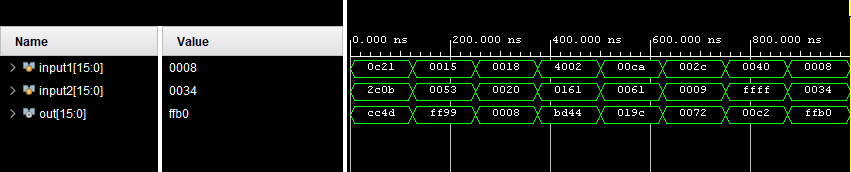
\includegraphics[width=0.5\textwidth]{part7_sim.png}
    \caption{16-bit 3A-2B Calculator Simulation}
\end{figure}


\section{DISCUSSION [25 points]}
\subsection{Preliminary} 
\begin{enumerate}
\item We will explain signed and unsigned addition for binary numbers in 2's complement notation.\\ 
On addition operation, 2's complement only used for negative numbers. Because we do not need to change the sign when adding unsigned binary numbers. For example: If we want to operate $4 + (-5)$ on signed 4-bit binary numbers we must be used 2's complement for create $(-5)$ in 4-bit binary.\\
$(0101)_2 = 5_1_0$  $\longrightarrow$ $(1011)_2 = (-5)_1_0$

\item We will explain signed and unsigned subtraction for binary numbers in 2’s complement notation.\\
2's complement used every subtraction operation on unsigned numbers. On signed numbers 2's complement only negative numbers. We don't need in used 2's complement for $2 - (-3)$  because this operation equals that $2 + 3$.

\item We will explain what carry, borrow and overflow mean, when they occur and how are they interpreted.
\begin{enumerate}
\item Carry is the result of the addition of two n-bit unsigned numbers can be a (n+1)-bit number.$(n+1)^th$ bit is called the carry. It can be occur in only  the addition of unsigned numbers.
\item Borrow can occur in the subtraction of unsigned numbers. The condition of being a borrow that first number is smaller than the second one.
\item Overflow can occur on only signed number. Occur in both addition and subtraction operations. It is determined by looking at the sign of the numbers added or subtracted and the sign of the result. If there is an operation overflow, that operation cannot be represented. There is an overflow in the following cases:\\
pos. + pos. $\longrightarrow$ neg. \hspace{1cm}  pos. - neg.$\longrightarrow$ neg.\\ neg. + neg. $\longrightarrow$ pos. \hspace{1cm} neg. - pos. $\longrightarrow$ pos.

\end{enumerate}

\end{enumerate}

\subsection{PART1}

In PART 1 we need to implement AND, OR, NOT, XOR gates as modules. Codes of these modules given below.

\begin{lstlisting}[language = Verilog]

    //and gate assign
    assign out = input1 & input2; 
    
    //not gate assign
    assign out = ~input1;

    //or gate assign
    assign out = input1 | input2;


\end{lstlisting}
For the whole circuit the module is given below.

\subsection{PART2}
In this part we are implementing 1-Bit Half Adder module using AD,OR,NOT,XOR modules we designed previously.

Code for the 1-Bit Half Adder is below.

\begin{lstlisting}[language = Verilog]
    module halfadder(
        input input1,
        input input2,
        output sum,
        output carry
    );
        xorgate xor1(.input1(input1), .input2(input2), .out(sum));
        andgate and1(.input1(input1), .input2(input2), .out(carry));
    endmodule
\end{lstlisting}


\subsection{PART3}
In this part we are implementing 1-Bit Full Adder module using AD,OR,NOT,XOR and 1-Bit half adder modules we designed previously.

Code for the 1-Bit Full Adder is below.

\begin{lstlisting}[language = Verilog]

    module fulladder(
        input input1,
        input input2,
        input inputc,
        output outc,
        output sum
    );
        wire araKablo1;//first sum
        wire araKablo2; //first carry
        wire araKablo3; // second carry
    
        halfadder ha1( .input1(input1), .input2(input2), .sum(araKablo1), .carry(araKablo2));
        halfadder ha2( .input1(araKablo1), .input2(inputc), .sum(sum), .carry(araKablo3));
        orgate or1(.input1(araKablo2), .input2(araKablo3), .out(outc));
    endmodule
\end{lstlisting}

\subsection{PART4}
In this part we are implementing 4-Bit Full Adder module using AD,OR,NOT,XOR and 1-Bit Full Adder modules we designed previously.

Code for the 4-Bit Full Adder is below.

\begin{lstlisting}[language = Verilog]

    module fulladder4bit(
        input [3:0] input1,
        input [3:0] input2,
        input inputc,
        output outc,
        output [3:0] sum
    );
        wire [2:0] araKablo;
    
        fulladder fa1( .input1(input1[0]),  .input2(input2[0]), .inputc(inputc), .outc(araKablo[0]), .sum(sum[0])  );
        fulladder fa2( .input1(input1[1]),  .input2(input2[1]), .inputc(araKablo[0]), .outc(araKablo[1]), .sum(sum[1])  );
        fulladder fa3( .input1(input1[2]),  .input2(input2[2]), .inputc(araKablo[1]), .outc(araKablo[2]), .sum(sum[2])  );
        fulladder fa4( .input1(input1[3]),  .input2(input2[3]), .inputc(araKablo[2]), .outc(outc), .sum(sum[3])  );
    
    endmodule
\end{lstlisting}


\subsection{PART5}
In this part we are implementing 16-Bit Full Adder module using AD,OR,NOT,XOR and 4-Bit Full Adder modules we designed previously.

Code for the 16-Bit Full Adder is below.

\begin{lstlisting}[language = Verilog]

module fulladder16bit(
    input [15:0] input1,
    input [15:0] input2,
    input inputc,
    output outc,
    output [15:0] sum
);
    wire [2:0] araKablo;
    fulladder4bit fafour1( .input1(input1[3:0]),  .input2(input2[3:0]), .inputc(inputc), .outc(araKablo[0]), .sum(sum[3:0])  );
    fulladder4bit fafour2( .input1(input1[7:4]),  .input2(input2[7:4]), .inputc(araKablo[0]), .outc(araKablo[1]), .sum(sum[7:4])  );
    fulladder4bit fafour3( .input1(input1[11:8]),  .input2(input2[11:8]), .inputc(araKablo[1]), .outc(araKablo[2]), .sum(sum[11:8])  );
    fulladder4bit fafour4( .input1(input1[15:12]),  .input2(input2[15:12]), .inputc(araKablo[2]), .outc(outc), .sum(sum[15:12])  );
endmodule

\end{lstlisting}

\subsection{PART5}
In this part we are implementing 16-Bit Full Adder module using AD,OR,NOT,XOR and 4-Bit Full Adder modules we designed previously.

Code for the 16-Bit Full Adder is below.

\begin{lstlisting}[language = Verilog]

module fulladder16bit(
    input [15:0] input1,
    input [15:0] input2,
    input inputc,
    output outc,
    output [15:0] sum
);
    wire [2:0] araKablo;
    fulladder4bit fafour1( .input1(input1[3:0]),  .input2(input2[3:0]), .inputc(inputc), .outc(araKablo[0]), .sum(sum[3:0])  );
    fulladder4bit fafour2( .input1(input1[7:4]),  .input2(input2[7:4]), .inputc(araKablo[0]), .outc(araKablo[1]), .sum(sum[7:4])  );
    fulladder4bit fafour3( .input1(input1[11:8]),  .input2(input2[11:8]), .inputc(araKablo[1]), .outc(araKablo[2]), .sum(sum[11:8])  );
    fulladder4bit fafour4( .input1(input1[15:12]),  .input2(input2[15:12]), .inputc(araKablo[2]), .outc(outc), .sum(sum[15:12])  );
endmodule

\end{lstlisting}


\subsection{PART6}
In this part we are implementing 16-Bit Full Adder-Substractor module using AD,OR,NOT,XOR and 16-Bit Full Adder modules we designed previously.

We also designed a 16-bit XOR gate for the second input. Code sample from the 16-bit XOR gate is below. We implemented the same logic for all 16 bits.

\begin{lstlisting}[language = Verilog]
module xorla(
    input [15:0] input1,
    input I,
    output [15:0] out
    );
    xorgate XOR0(.input1(input1[0]),.input2(I),.out(out[0]));
\end{lstlisting}

Code for the 16-Bit Full Adder-Substractor is below. We only added inputs and the logic here. We receive an input to determine if number is signed.

\begin{lstlisting}[language = Verilog]

module addersubstractor16bit(
    input S,
    input I,
    input [15:0] input1,
    input [15:0] input2,
    output [15:0] sum,
    output borrow,
    output overflow,
    output outc,
    output isValid
);
    wire [15:0] araKablo1;
    xorla XOR1(.input1(input2),.I(I),.out(araKablo1));
    fulladder16bit FA16(.input1(input1),.input2(araKablo1),.inputc(I),.outc(outc),.sum(sum));
    //flag logic below
\end{lstlisting}

To determine if there is borrow or overflow we designed a flag logic. Based on the sum and cout we determine if there is overflow or borrow.

\begin{lstlisting}[language = Verilog]
    andgatethreeinput AND1(.input1(araKablo2), .input2(araKablo3), .input3(sum[0]), .out(araKablo7)); // A_0' and B_0' and SUM_0
    andgatethreeinput AND2(.input1(input1[0]), .input2(input2[0]), .input3(araKablo4), .out(araKablo8)); //A_0 and B_0 and SUM_0'
    andgatethreeinput AND3(.input1(araKablo2), .input2(input2[0]), .input3(sum[0]), .out(araKablo9)); //A_0' and B_0 and SUM_0
    andgatethreeinput AND4(.input1(input1[0]), .input2(araKablo3), .input3(araKablo4), .out(araKablo10)); //A_0 and B_0' and SUM_0'
    
    orgate OR1(.input1(araKablo7), .input2(araKablo8), .out(araKablo11)); 
    orgate OR2(.input1(araKablo9), .input2(araKablo10), .out(araKablo12));

    andgatethreeinput AND5(.input1(S), .input2(araKablo6), .input3(araKablo11), .out(araKablo13));
    andgatethreeinput AND6(.input1(S), .input2(I), .input3(araKablo12), .out(araKablo14));
    
    orgate OR3(.input1(araKablo13), .input2(araKablo14), .out(overflow));

    andgatethreeinput AND7(.input1(I),.input2(araKablo5),.input3(outc),.out(borrow));
    
    orgate VALID(.input1(overflow),.input2(borrow),.out(isValid));
\end{lstlisting}

\subsection{PART7}
In this part we are implementing a module calculates 3A-2B using the modules we designed previously. We receive A and B, then we obtain 3A and 2B by using 16-bit Full Adder/Substractor. In the end we calculate 3A-2B using the same module.

\begin{lstlisting}[language = Verilog]

module part7(
    input [15:0] input1,
    input [15:0] input2,
    output [15:0] out
   
    );
    wire [15:0] twoA,threeA,twoB;
    addersubstractor16bit TWOA(.input1(input1),.input2(input1),.S(0),.I(0),.sum(twoA));//2a
    addersubstractor16bit THREEA(.input1(twoA),.input2(input1),.S(0),.I(0),.sum(threeA));//3a
    
    addersubstractor16bit TWOB(.input1(input2),.input2(input2),.S(0),.I(0),.sum(twoB));//2b
    
    addersubstractor16bit result(.input1(threeA),.input2(twoB),.S(0),.I(1),.sum(out));//2a

endmodule

\end{lstlisting}


\section{CONCLUSION [10 points]}
While examining the overflow situation, we noticed that there was a lack of resources. There was no information about the overflow circuit in the referenced source either. We realized that 16-Bit Full Adder-Subtractor design only stretched the assignment. We think that designing an 8-Bit Full Full Adder- Substractor or 4-Bit Full Full Adder- Substractor can teach the same thing.

\newpage
\addcontentsline{toc}{section}{\numberline {}REFERENCES}

\bibliographystyle{unsrt}
\bibliography{reference}

\end{document}

